\documentclass[tikz]{standalone}
\usepackage{amsmath}
\definecolor{bg}{HTML}{171D2B}
\definecolor{aksen}{HTML}{F7B538}
\definecolor{halus}{HTML}{2A3350}
\begin{document}
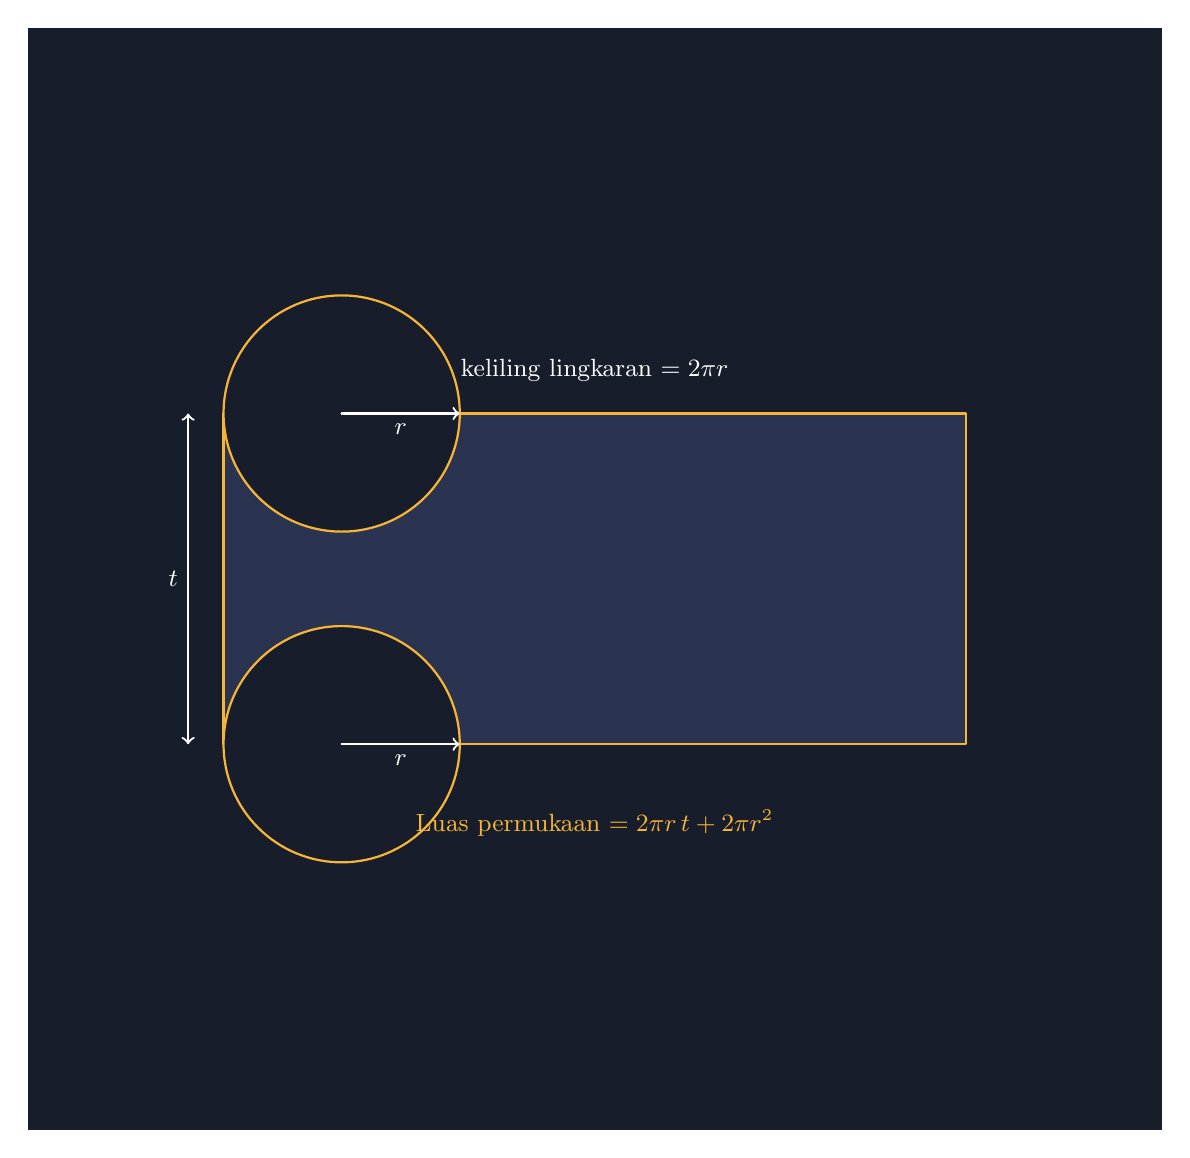
\begin{tikzpicture}[x=1cm,y=1cm, line cap=round, line join=round]
  \fill[bg] (-7.2,-7.0) rectangle (7.2,7.0);
  % --- net of a cylinder: rectangle r wide, h tall, plus two circles
  % r=2.3 (so rect width = 2*pi*r = 14.45 too wide) -> use r=1.5, width=9.42
  \def\r{1.5}
  \pgfmathsetmacro{\w}{2*pi*\r}
  \def\h{4.2}
  % rectangle (lateral surface), placed centered at origin
  \draw[thick, aksen, fill=halus] (-\w/2,-\h/2) rectangle (\w/2,\h/2);
  % attach circles (radius r) centered on the long sides
  \draw[thick, aksen, fill=bg] (-\w/2+\r, \h/2) circle (\r);
  \draw[thick, aksen, fill=bg] (-\w/2+\r,-\h/2) circle (\r);
  % radius markers
  \draw[thick, white, ->] (-\w/2+\r,\h/2) -- (-\w/2+2*\r,\h/2) node[midway, below, text=white, font=\small] {$r$};
  \draw[thick, white, ->] (-\w/2+\r,-\h/2) -- (-\w/2+2*\r,-\h/2) node[midway, below, text=white, font=\small] {$r$};
  % height label on rectangle
  \draw[thick, white, <->] (-\w/2-0.45,-\h/2) -- (-\w/2-0.45,\h/2) node[midway, left, text=white, font=\small] {$t$};
  % width label = 2 pi r
  \node[text=white, font=\small] at (0,\h/2+0.55) {keliling lingkaran $= 2\pi r$};
  \node[text=aksen, font=\small] at (0,-\h/2-1.0) {Luas permukaan $= 2\pi r\,t + 2\pi r^2$};
\end{tikzpicture}
\end{document}
